\section{How we are going to do it}
	This section will give a brief description of how we plan on implementing our solution. 
	
	\subsection{Central Datastore}
		We propose creating a central datastore containing all public information about NTNU. We will provide APIs that will give easy access to all the data, and the APIs will be open to the public. 
		% Tenk IME-API!
NUDL will use this datastore, illustrated in Figure \ref{fig:datastore}, to retrieve all necessary information about courses, rooms and timetables, and so it will need to be constantly updated in order to contain the most recent information. This means that third party developers will have equal access to non-restricted data, which will enable students and staff to write their own tools which can easily be integrated with NUDL. We aim to make NUDL a platform to which tools can be added and removed as needed, not a monolithic system where someone else is in control. The calendar generator at \url{www.ntnu.1024.no} is a great example of an extremely useful application created by a student. We know that IME offers some APIs today, and these could be extended and integrated into our system.
\begin{figure}[h]
\centering
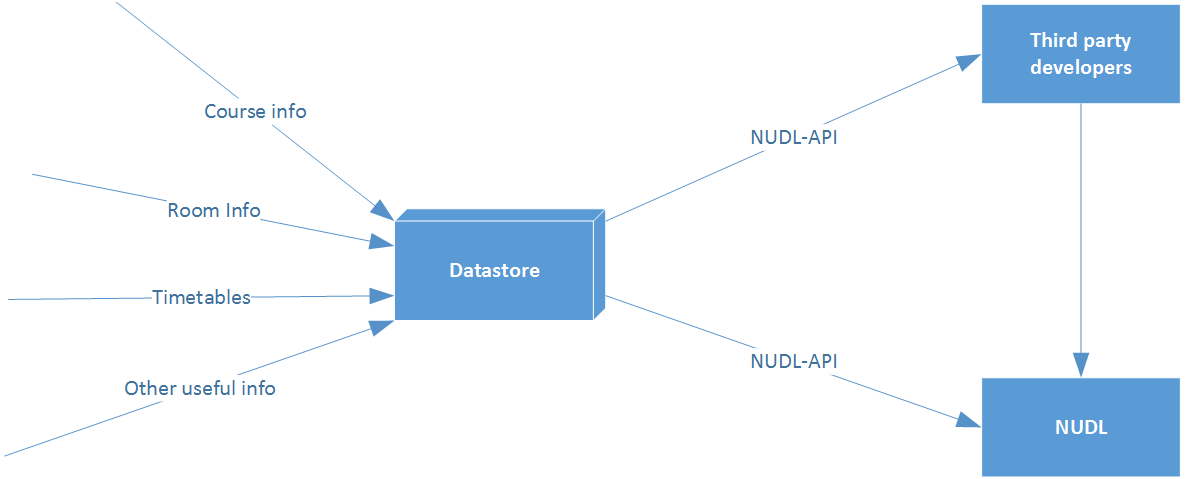
\includegraphics[width = \textwidth]{datastore}
\caption{Datastore and APIs}
\label{fig:datastore}
\end{figure}

	\subsection{Storage model}
		The datastore mentioned in the previous section will only contain publicly available information. In addition, we will have two other separate databases; one userstore containing information about staff and students, and one database storing everything related to the individual courses. In Figure \ref{fig:storagemodel} the general datastore is shown on the left, course database in the middle and userstore on the right. The dotted green circle means that everyone is given read access, a full red circle means read and write access is restricted to a strict subset of users, and a full green circle means that there are two different levels of security. The userstore will be fully secured against unauthorized access, and only the users will have access to their individual information. The course database will be used to supply the same functionality as It's Learning does today. Students will for the most part have read-only access to the course database, but they will be given the possibility to deliver exercises and participate in forums and chat. Course staff will have read and write access to the course content pages, but will only be able to read the student submissions. Administrative staff will have accesses as needed. 
Course staff will be able to make course material available to non-students, by making it accessible through the public APIs. 
\begin{figure}
\centering
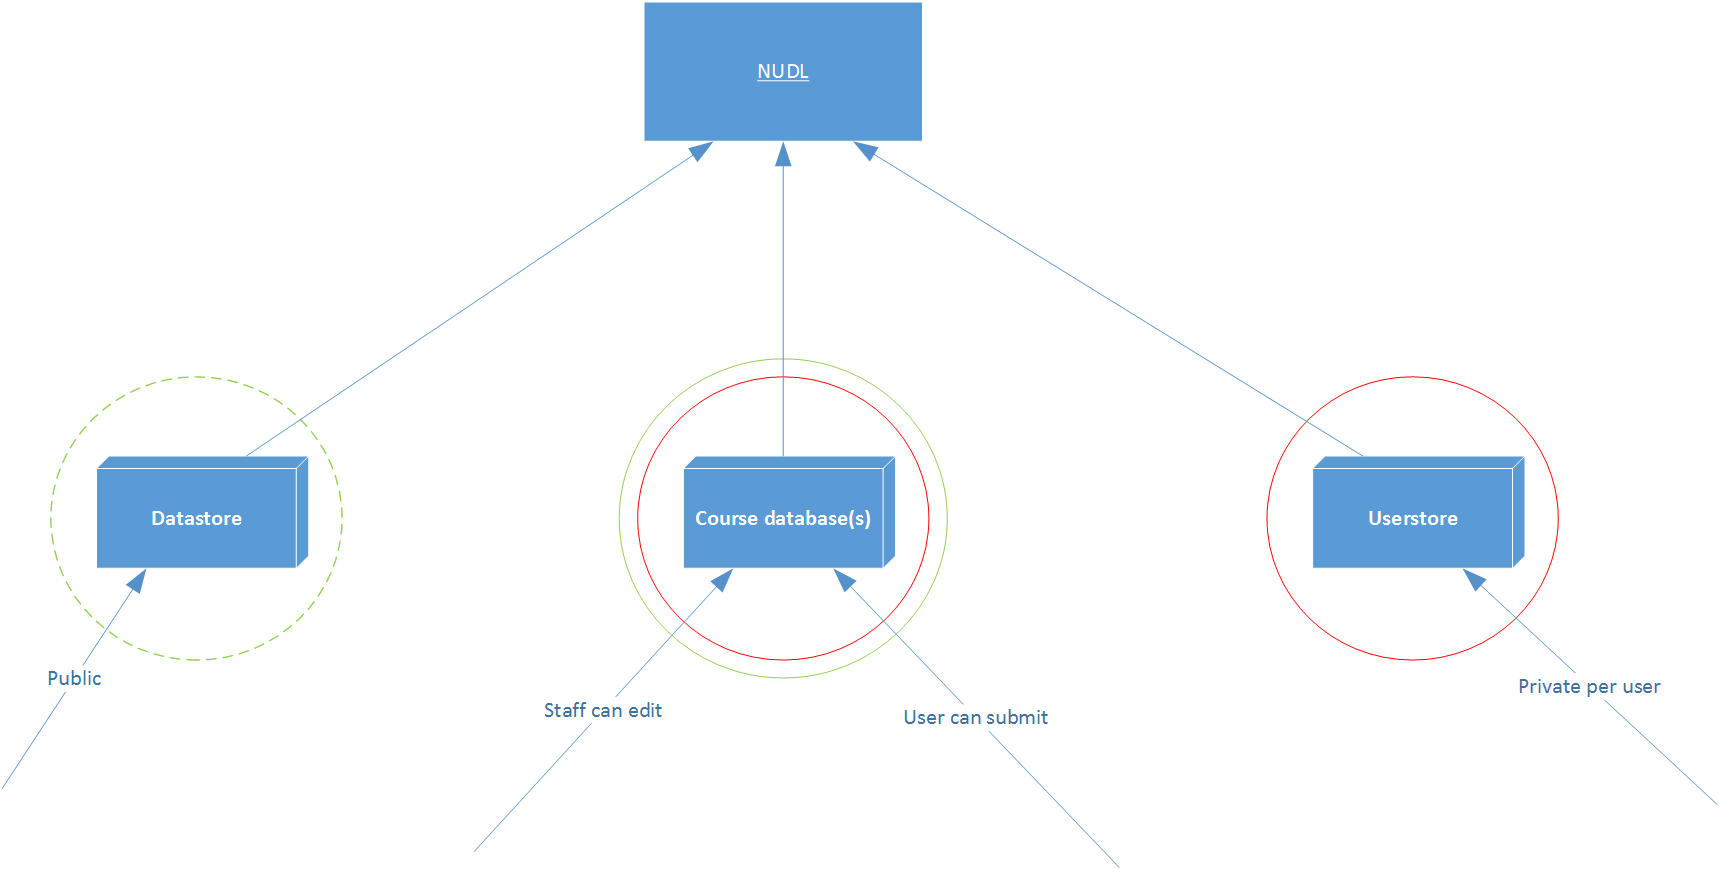
\includegraphics[width = \textwidth]{moreStorage}
\caption{Storage model}
\label{fig:storagemodel}
\end{figure}

		
	\subsection{User interface} 
		We want NUDL to present users with a user-friendly and unified interface. It will not be like today, where you have different interfaces for It's Learning, Studweb and Eksamensweb. It's Learning and Eksamensweb will be replaced by NUDL, and Studweb will be hidden from view. Students can log in to Studweb from NUDL, via Feide, but they will be met by the NUDL interface, which will take care of the communication with Studweb, as shown in Figure \ref{fig:layers}. Staff and students can do everything they need to do, from one central location. There will be no more need to log in to different services like today, where one first has to search for courses on ntnu.no, (UI no.1) log on to Studweb in order to register for the course (navigating a very cluttered and confusing UI no.2) and then log on to Innsida (UI no.3) and then finally continue to It's Learning (UI no.4). If they want to complain on a grade, they need to send in a paper form, or students at IDI can log on to Eksamensweb (UI no.5). NUDL combines all these different interfaces into one coherent whole. 
\begin{figure}
\centering
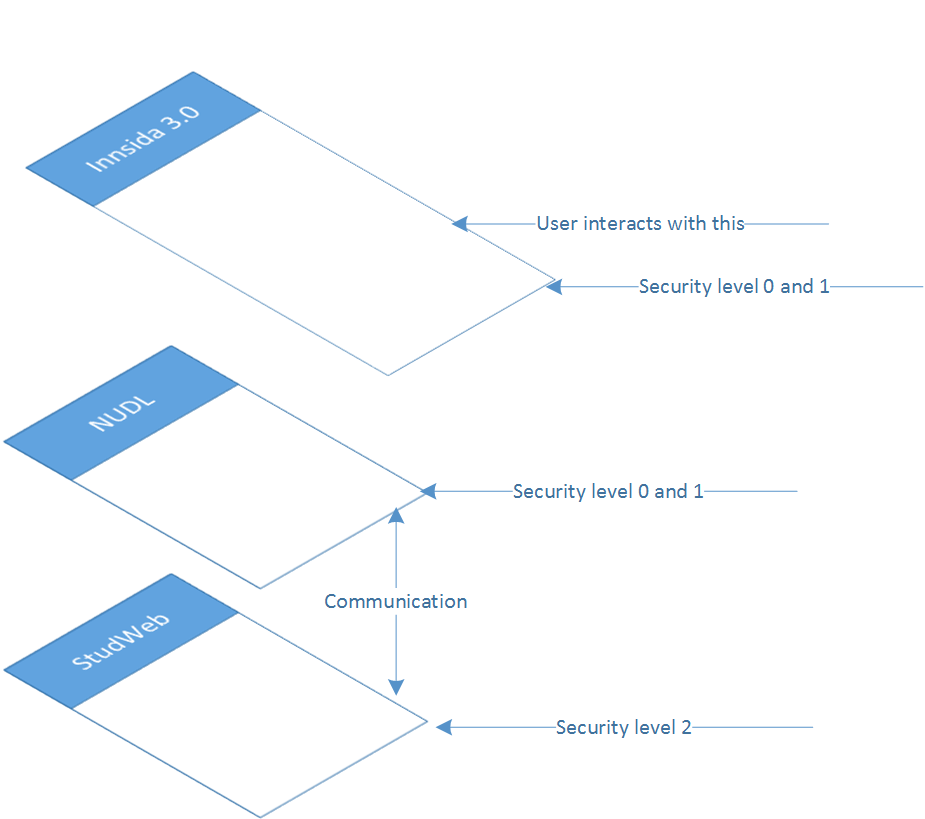
\includegraphics[width = \textwidth]{Layers}
\caption{Layered architecture}
\label{fig:layers}
\end{figure}